\section{H. 볼링장 아르바이트}

\begin{frame} % No title at first slide
    \sectiontitle{H}{볼링장 아르바이트}
    \sectionmeta{
        \texttt{ad\_hoc, sorting}\\
        출제진 의도 -- \textbf{\color{acgold}Hard}
    }
    \begin{itemize}
        \item 출제자: 이승엽\textsuperscript{\color{kupc-gray}\texttt{delena0702}}
    \end{itemize}
\end{frame}

\begin{frame}{\textbf{H}. 볼링장 아르바이트}
	\begin{itemize}
		\item 모든 볼링공을 정렬하기 위해서는 각 볼링공마다 최대 1번만 이동하면 정렬할 수 있습니다.
		\item 예시로 가장 무거운 공을 제외한 나머지 볼링공을 무거운 순서대로 이동하면 $N - 1$번에 정렬할 수 있습니다.
		\item 따라서 반드시 이동이 필요한 볼링공들의 개수를 세면 최소 이동 횟수를 구할 수 있습니다.
	\end{itemize}
\end{frame}

\begin{frame}{\textbf{H}. 볼링장 아르바이트}	
	\begin{itemize}
		\item 최소 이동 횟수로 볼링공을 정렬하기 위해서는 가장 무거운 공보다 뒤에 있는 공들은 반드시 이동해야 합니다.
		\item 그다음으로, 2번째로 무거운 공과 1번째로 무거운 공 사이의 모든 공이 이동해야 하고, 3번째와 2번째 사이 역시 마찬가지입니다.
		\item 이때, 만약 2번째로 무거운 공이 1번째로 무거운 공보다 뒤에 있다면, 이미 배열의 앞으로 이동할 예정이므로 1번째 무거운 공 앞의 모든 공들이 이동해야 하는 공이 됩니다.
	\end{itemize}
\end{frame}

\begin{frame}{\textbf{H}. 볼링장 아르바이트}	
	\begin{figure}[h!]
		\centering
		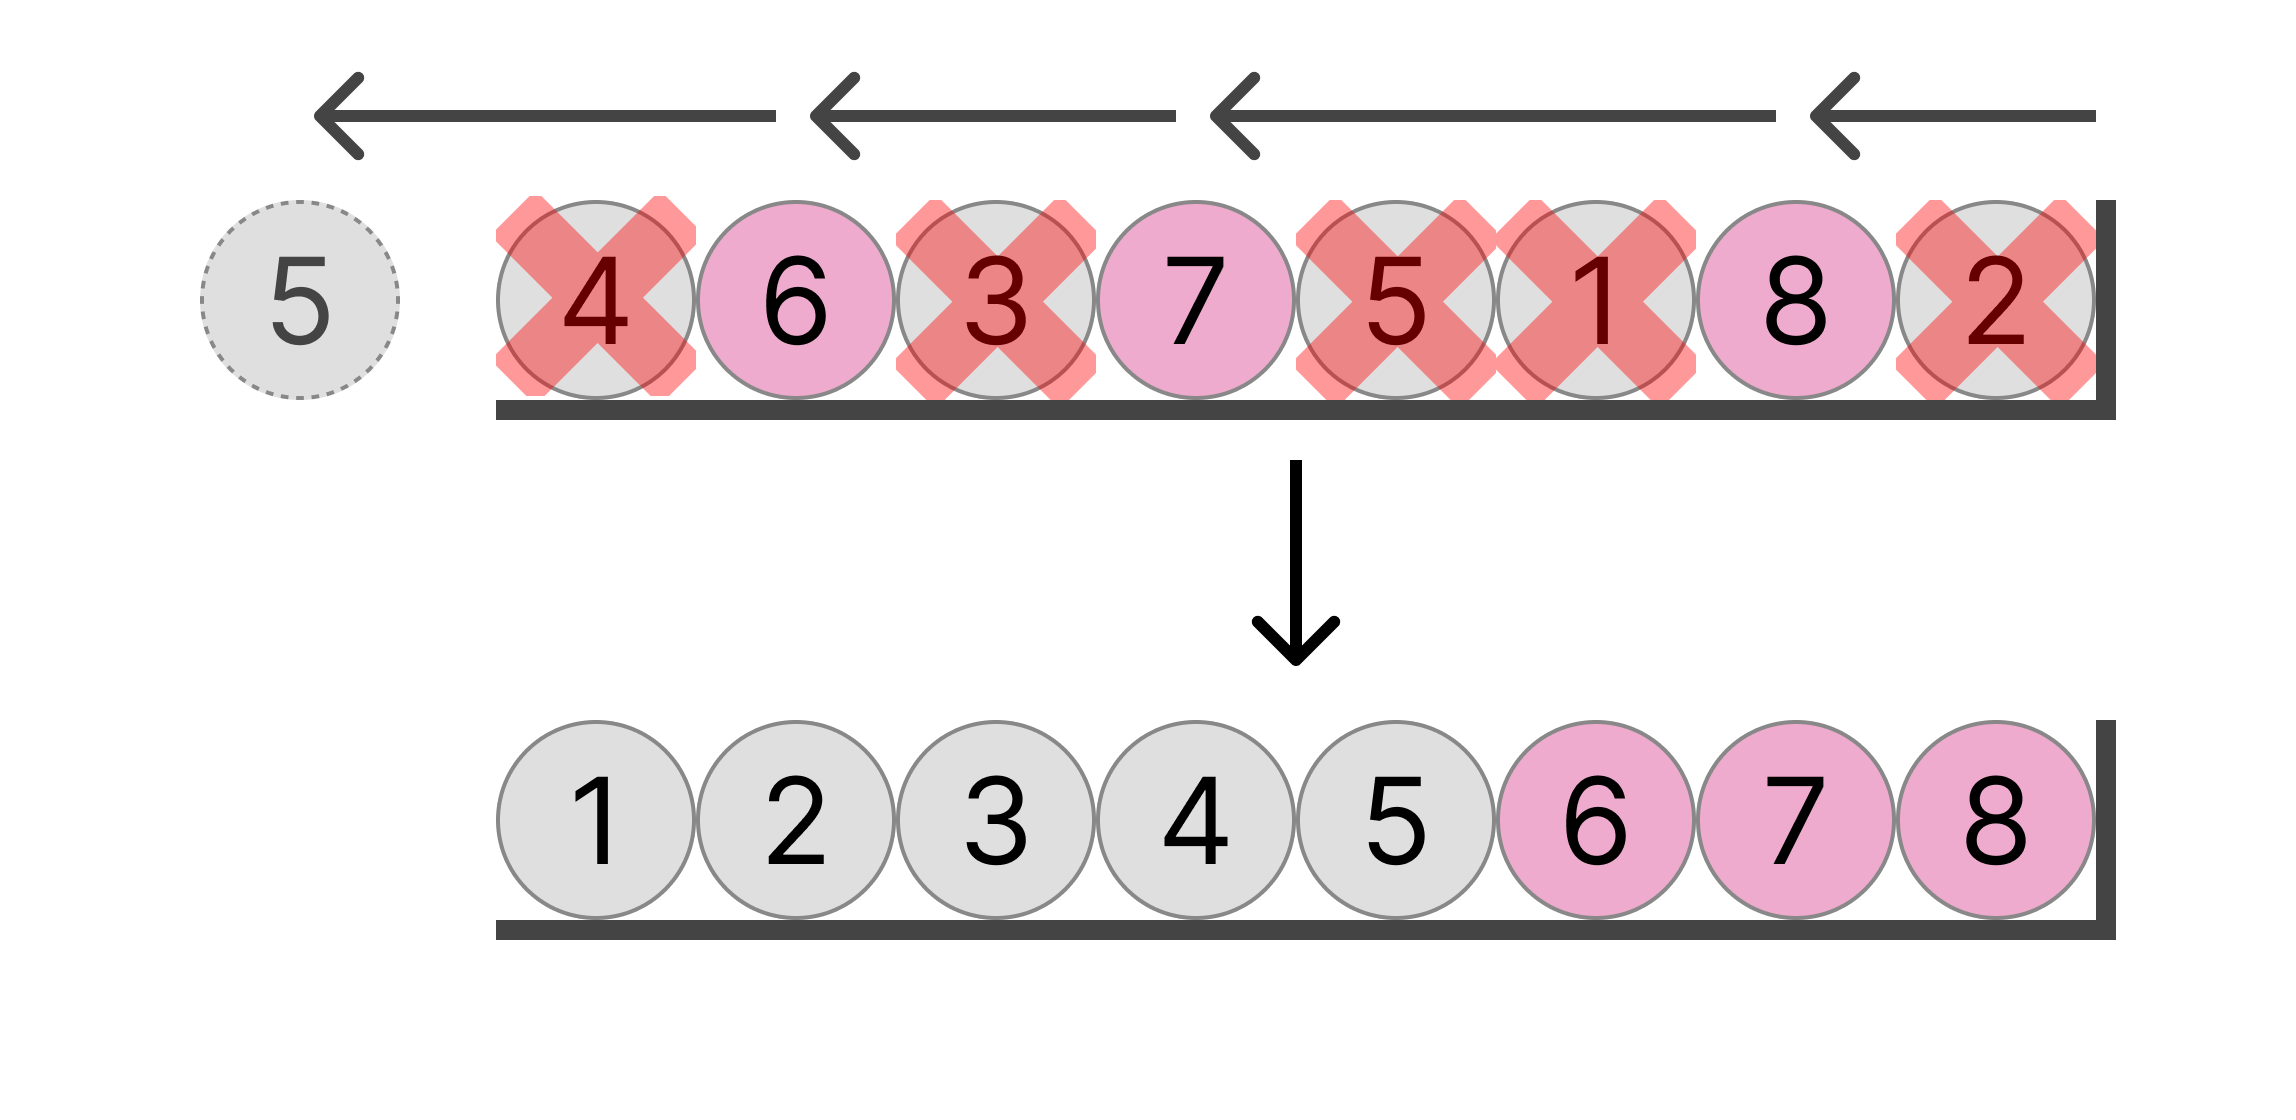
\includegraphics[width=0.9\linewidth]{../images/bowling-part-time/1.png}
	\end{figure}
\end{frame}

\begin{frame}{\textbf{H}. 볼링장 아르바이트}
	\begin{itemize}
		\item 이렇게 모든 공들을 확인할 때까지 공이 무거운 순서대로 확인하게 된다면, 반드시 이동해야 할 공들의 개수를 구할 수 있습니다.
		\item 따라서 원래 배열에서 역순으로 탐색하여 가장 무거운 공부터 순서대로 몇 개가 있는지 확인하면, 이동할 필요가 없는 공의 개수를 구할 수 있습니다.
		\item 따라서 답은 $N - $[이동할 필요가 없는 공의 개수] 입니다.
		\item 이 풀이의 시간복잡도는 정렬하는데 걸리는 시간인 \complexity{N \log N} 입니다.
	\end{itemize}
\end{frame}